\section{Conventions used in this document}
\label{sec:conventions}


%% UML
\subsection{UML Classes}
\label{sec:umlconventions}
A SED-ML UML class (\fig{umlClass}) consists of a class name (\code{ClassName}) and a number of attributes (\code{attribute}) each of a specific data type (\code{type}). The SED-ML UML specification does not make use of UML \code{operations}.
\begin{figure}[h]
\centering
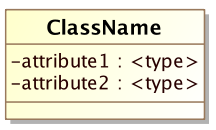
\includegraphics[width=0.2\textwidth]{images/uml/umlClass.png}
\caption{SED-ML UML Class with class names and attributes}
\label{fig:umlClass}
\end{figure}

SED-ML class names always begin with upper case letters. If they are composed of different words, the camel case style is used, as in e.\,g.\ \code{DataGenerator}.

\subsection{UML Relationships}
%% RELATIONS
\subsubsection{UML Relation Types}
\begin{figure}[h]
\centering
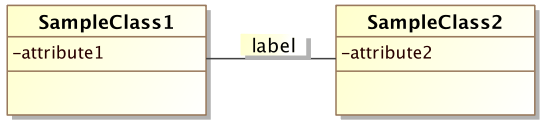
\includegraphics[width=0.5\textwidth]{images/uml/classRelation.png}
\caption{UML Class connectors}
\label{fig:umlConnectors}
\end{figure}

Links between classes specify the connection of objects with each other (\fig{umlConnectors}). The different relation types used in the SED-ML specification include aggregation, composite aggregation, and generalisation. The label on the line is called symbol (\code{label}) and describes the relation of the objects of both classes. 

%% Association
The \concept{association} (\fig{umlAssociation}) indicates the existence of a connection between the objects of the participating classes. Often associations are directed to show how the label should be read (in which direction). Associations can be uni-directional (one arrowhead), or bidirectional (zero or two arrowheads). 
\begin{figure}[h]
\centering
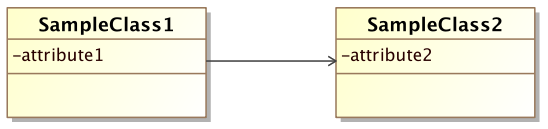
\includegraphics[width=0.5\textwidth]{images/uml/umlAssociation.png}
\caption{UML Association}
\label{fig:umlAssociation}
\end{figure}

 
%% Aggregation
The \concept{aggregation} (\fig{umlAggregation}, top) indicates that the objects of the participating classes are connected in a way that one class (\code{Whole}) consists of several parts (\code{Part}). In an aggregation, the parts may be independent of the whole. For example, a car (\code{Whole})  has several parts called wheel (\code{Part}); however, the wheels can exist independently of the car while the car requires the wheels in order to function.
\begin{figure}[h]
\centering
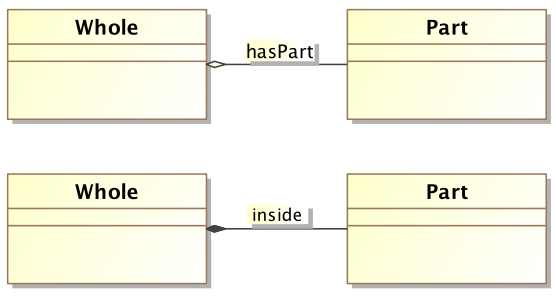
\includegraphics[width=0.5\textwidth]{images/uml/umlAggregation.png}
\caption{UML Aggregation}
\label{fig:umlAggregation}
\end{figure}

%% Composite Aggregation
The \concept{composite aggregation} (\fig{umlAggregation}, bottom) indicates that the objects of the participating classes are connected in a way that one class (\code{Whole}) consists of several parts (\code{Part}). In contrast to the aggregation, the subelements (\code{Part}) are dependent on the parent class (\code{Whole}). An example is that a university (\code{Whole}) consists of a number of departments (\code{Part}) which have a so-called ``lifetime responsibility'' with the university, e.\,g.\ if the university vanishes,  the departments will vanish with it \citep{Bel03}.

%% Inheritance
The \concept{generalisation} (\fig{umlGeneralisation}) allows to extend classes (\code{BaseClass}) by additional properties. The derived class (\code{DerivedClass}) inherites all properties of the base class and defines additional ones. In the given example, an instance of \code{DerivedClass} has two attributes \code{attribute1} and \code{attribute2}.
%
\begin{figure}[h]
\centering
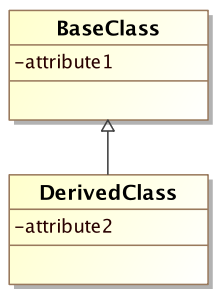
\includegraphics[width=0.2\textwidth]{images/uml/umlGeneralisation.png}
\caption{UML Generalisation}
\label{fig:umlGeneralisation}
\end{figure}
%
%% CARDINALITIES
\subsubsection{UML multiplicity}
UML multiplicity defines the number of objects in one class that can be related to one object in the other class (also known as \concept{cardinality}). Possible types of multiplicity include values (1), ranges (1$..$4), intervals (1,3,9), or combinations of ranges and intervals. The standard notation for ``many'' is the asterix (*). 

Multiplicity can be defined for both sides of a relationship between classes. The default relationship is ``many to many''. 
The example in \fig{umlMulti} expresses that a class is given by a professor, and a professor might give one to many classes.
\begin{figure}[h]
\centering
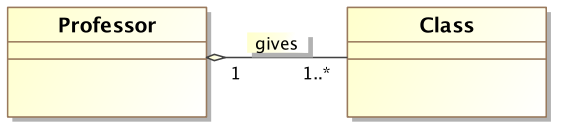
\includegraphics[width=0.4\textwidth]{images/uml/umlMultiplicity.png}
\caption{UML Multiplicity in an Aggregation}
\label{fig:umlMulti}
\end{figure}

%% XML SCHEMA
\subsection{XML Schema language elements}
The main building blocks of an XML Schema specification are:
\begin{itemize}
\item {simple and complex types}
\item {element specifications}
\item {attribute specifications}
\end{itemize}
XML Schema \concept{definitions} create new types, \concept{declarations} define new elements and attributes.
The definition of new (simple and complex) types can be based on a number of already existing, prefedined types (string, boolean, float). Simple types are restrictions or extensions of predefined types. Complex types describe how attribues can be assigned to elements and how elements can contain further elements. The current SED-ML XML Schema only makes use of \emph{complex type definitions}.
An example for a complex type definition is given in listing \ref{lst:complexType}:
%
\begin{myXmlLst}{Complex Type definition of the SED-ML \code{computeChange} element}{lst:complexType}
<xs:element name="computeChange">
		<xs:complexType>
			<xs:complexContent>
				<xs:extension base="SEDBase">
					<xs:sequence>
						<xs:element ref="listOfVariables" minOccurs="0" />
						<xs:element ref="listOfParameters" minOccurs="0" />
						<xs:element ref="math" />
					</xs:sequence>
					<xs:attribute name="target" use="required" type="xs:token" />
				</xs:extension>
			</xs:complexContent>
		</xs:complexType>
	</xs:element>
\end{myXmlLst}
%
It shows the declaration of an element called \code{computeChange} that is used in SED-ML to change mathematical expressions. The element is defined using an \emph{unnamed} complex type which is build of further elements called \code{listOfVariables}, \code{listOfParameters}, and \code{math}. 
Additionally, the element \code{computeChange} has an attribute \code{target} declared. Please note that the definition of the elements inside the complex type are only referred to and will be found elsewhere in the schema.

The nesting of elements in the schema can be expressed using the \code{xs:sequence} (a sequence of elements), \code{xs:choice} (an alternative of elements to choose from), or \code{xs:all} (a set of elements that can occur in any order) concepts. The current SED-ML XML Schema only uses the \emph{sequence} of elements. 

\subsubsection{Multiplicities}
The standard multiplicity for each defined \code{element} is 1. Explicit multiplicity is to be defined using the \code{minOccurs} and \code{maxOccurs} attributes inside the complex type definition, as shown in listing \ref{lst:multiplicity}.

\begin{myXmlLst}{Multiplicity for complex types in XML Schema}{lst:multiplicity}
<xs:element name="dataGenerator">
		<xs:complexType>
			<xs:complexContent>
				<xs:extension base="SEDBase">
					<xs:sequence>
						<xs:element ref="listOfVariables" minOccurs="0" />
						<xs:element ref="listOfParameters" minOccurs="0" />
						<xs:element ref="math" />
					</xs:sequence>
					<xs:attributeGroup ref="idGroup" />
				</xs:extension>
			</xs:complexContent>
		</xs:complexType>
	</xs:element>
\end{myXmlLst}
%
In this example, the \code{dataGenerator} type is build of a sequence of three elements: The \code{listOfVariables} element is not necessary for the definition of a valid \code{dataGenerator} XML structure (it may occur 0 times or once). The same is true for the \code{listOfParameters} element (it may as well occur 0 times or once). The \code{math} element, however, uses the implicit standard multiplicity -- it must occur exactly 1 time in the \code{dataGenerator} specification.

\subsection{Type extensions}
XML Schema offers mechanisms to restrict and extend previously defined complex types. Extensions add element or attribute declarations to existing types, while restrictions restrict the types by adding further characteristics and requirements (facets) to a type. An example for a type extension is given in listing \ref{lst:xmlExtension}.
%
\begin{myXmlLst}{Definition of the sedML type through extension of SEDBase in SED-ML}{lst:xmlExtension}
	<xs:element name="sedML">
		<xs:complexType>
			<xs:complexContent>
				<xs:extension base="SEDBase">
					<xs:sequence>
						<xs:element ref="listOfSimulations" minOccurs="0" />
						<xs:element ref="listOfModels" minOccurs="0" />
						<xs:element ref="listOfTasks" minOccurs="0" />
						<xs:element ref="listOfDataGenerators" minOccurs="0" />
						<xs:element ref="listOfOutputs" minOccurs="0" />
					</xs:sequence>
					<xs:attribute name="level" type="xs:decimal" use="required"
						fixed="1" />
					<xs:attribute name="version" type="xs:decimal" use="required"
						fixed="1" />
				</xs:extension>
			</xs:complexContent>
		</xs:complexType>
	</xs:element>
\end{myXmlLst}
%
%% Q: How about renaming sedML to sed-ml for the next version?
The \code{sedML} element is an extension of the previously defined \code{SEDBase} type. It extends \code{SEDBase} by a sequence of five additional elements (\code{listOfSimulations}, \code{listOfModels}, \code{listOfTasks}, \code{listOfDataGenerators}, and \code{listOfOutputs}) and a new attribute \code{version}.

%% MAPPINGS
% \subsection{Mappings}

% \subsubsection{Mapping the Workflow Structure to a UML Class Diagram Structure}
% The main structure of the above shown workflow can be easily recognised in main class structure of the UML class diagram as shown in Figure \ref{fig:sedml}. Other processes of the workflow have been mapped to according class attributes and/or additional classes in the UML class diagram structure.

% \subsubsection{Conversion of UML into XML Schema}
% Also, the conversion of the UML class diagram representation into the XML Schema model is very intuitive and follows a small set of rules: UML Classes from the diagram are mapped to XML \alert{tbc}
% Page 6 of the SBML spec


%%% Local Variables: 
%%% mode: latex
%%% TeX-master: "../sed-ml-L1V1"
%%% End: 
